\documentclass[10pt,a4paper]{article}
\usepackage[utf8]{inputenc}
\usepackage{amsmath}
\usepackage{amsfonts}
\usepackage{amssymb}
\usepackage{mathtools}
\usepackage{amsthm}
\usepackage[ruled, linesnumbered]{algorithm2e}

\newtheorem*{theorem}{Theorem}
\theoremstyle{remark}
\newtheorem*{remark}{Remark}

\DeclarePairedDelimiter{\nint}\lfloor\rceil

\begin{document}
\title{Lattices}
\maketitle
\tableofcontents

\section{Silverman, Crypto}
\subsection{Lattices and Lattice Problems}
\subsubsection{What is a Lattice}
Let $\vec{v}_1,\ldots,\vec{v}_n\in\mathbb{R}^m$ be linearly independent vectors. The \emph{lattice L generated by $\vec{v}_1,\ldots,\vec{v}_n$} is the set of linear combinations
$$L=\{a_1\vec{v}_1+a_2\vec{v}_2+\ldots+a_n\vec{v}_n\vert a_1,\ldots,a_n\in\mathbb{Z}\}$$
Lattices have dimensions and bases just as vector spaces do. Bases of a lattice L are related by $GL(2,\mathbb{Z}$). We typically prefer lattices whose vectors have integer coordinates. Lattices are discrete additive subgroups of $\mathbb{R}^n$.

A lattice L with basis $\vec{v}_1,\ldots,\vec{v}_n$ has a \emph{fundamental domain} which is the set
$$\mathcal{F}(\vec{v}_1,\ldots,\vec{v}_n)=\{t_1\vec{v}_1,\ldots,t_n\vec{v}_n\vert 0\leq t_i\in\mathbb{R} < 1\}$$

A lattice $L\subset\mathbb{R}^n$ of dimension n, together with its fundamental domain, can tile $\mathbb{R}^n$. Specifically, for all $\vec{w}\in\mathbb{R}^n$,

$$\vec{w}=\vec{t} + \vec{v} \emph{ for a unique } \vec{t}\in\mathcal{F} \emph{ and a unique }\vec{v}\in L$$

The volume of the fundamental domain for a lattice L is called its \emph{volume} or \emph{determinant} and is denoted det(L). It's calculated using the determinant of the matrix which has basis vectors of L as its columns. You can prove this using integration and change of variables on the fundamental domain (cool).

det(L) is invariant for a lattice, i.e. it does not depend on the choice of fundamental domain or, similarly, choice of basis.

\subsubsection{Hard Lattice Problems}
There are two "fundamental" computational lattice problems:
\begin{enumerate}
\item \textbf{The Shortest Vector Problem (SVP)}: Find a nonzero vector $\vec{v}\in L$ which minimizes Euclidean norm $\vert\vert\vec{v}\vert\vert$. There may be more than one such vector.
\item \textbf{The Closest Vector Problem (CVP)}: Given a vector $\vec{w}\notin L$, find a vector $\vec{v}\in L$ which minimizes the Euclidean norm $\vert\vert \vec{w}-\vec{v}\vert\vert$. There may be more than one such vector.
\end{enumerate}
CVP is known to be $\mathcal{NP}$-hard, and SVP is $\mathcal{NP}$-hard when a "randomized reduction hypothesis" is imposed.

There is (often?) a correspondence between CVP in n dimensions and SVP in (n+1) dimensions.

\subsubsection{Practical Hard Lattice Problems}
Most $\mathcal{NP}$-hard/complete problems are difficult to utilize in generality, so we rely on subclasses of problems with desirable features such as efficiency or trapdoors. This can be dangerous, as these subclasses sometimes have vulnerabilities. Here are some examples
\begin{enumerate}
\item \textbf{Shortest Basis Problem (SBP)}: Find a basis $\vec{v}_1,\ldots,\vec{v}_n$ for a lattice that is shortest in some sense. Examples include minimizing $max\vert\vert \vec{v}_i\vert\vert_{1\leq i\leq n}$ or $\sum_{i=1}^n \vert\vert\vec{v}_i\vert\vert^2$.
\item \textbf{Approximate Shortest Vector Problem (apprSVP)}: Let $\psi(n)$ be a function of n. For a lattice L of dimension n, find a nonzero vector $\vec{v}\in L$ such that $\vert\vert \vec{v}\vert\vert \leq \psi(n)\vert\vert\vec{v}_{\text{shortest}}\vert\vert$.
\item \textbf{Approximate Closest Vector Problem (apprCVP)}: Same as apprSVP, but for CVP instead.
\end{enumerate}

\subsubsection{Questions}
\begin{itemize}
\item Is there a lattice with a finite base which is not a discrete group? NO
\item What can lattices with infinite bases look like?
\item Why are the SVP and CVP problems "fundamental?" are there other fundamental problems?
\item What is the "randomized reduction hypothesis" that makes SVP hard? (pg 395)
\item When can SVP and CVP be corresponded? When can they not be corresponded? (pg 395)
\item What makes a lattice problem (or general problem) practical or impractical? (pg 396)
\item Why is apprSVP phrased to handle multiple dimensions? It seems like it is a problem involving many lattices. (pg 396)
\item Does the fact that orthogonal lattices are easier to solve relate to the fact that we like reducing BQFs to orthogonal lattices? Does this relate to when BQFs are easy to solve? (pg 403)
\end{itemize}

\subsection{What Do We Know About Lattice Problems?}

\subsubsection{Bounds on Shortest Nonzero Vectors}
\begin{theorem}[Hermite's Theorem]
Every lattice L of dimension n contains a nonzero vector $\vec{v}\in L$ satisfying
$$\vert \vert \vec{v} \vert \vert\leq \sqrt{n}\textup{det}(L)^{1/n}$$
\end{theorem}
\begin{remark}
For a dimension n, we define \textit{Hermite's constant} $\gamma_n$ as the smallest value such that every lattice L of dimension n contains a nonzero vector $\vec{v}\in L$ satisfying
$$\vert \vert \vec{v} \vert \vert\leq \gamma_n\textup{det}(L)^{2/n}$$
and Hermite's theorem specifies $\gamma_n<n$.
\end{remark}
$\gamma_n$ is only known for $1\leq n \leq 8$ and for $n=24$.
For large values of $n$ Hermite's constant satisfies
$$\frac{n}{2\pi e} \leq \gamma_n \leq \frac{n}{\pi e}$$

The following theorem is used in proving Hermite's theorem.
\begin{theorem}[Minkowski's Theorem]
Let $L\subset \mathbb{R}^n$ be a lattice of dimension n and let $S\subset \mathbb{R}^n$ be a bounded symmetric convex set whose volume satisfies
$$\textup{Vol}(S)>2^n\textup{det}(L)$$
Then S contains a nonzero lattice vector. If S is also closed, then it suffices to take $\textup{Vol}(S)\geq 2^n \textup{det}(L)$.
\end{theorem}

Hermite's theorem can be improved using hyperspheres and the gamma function. We do not explore this here.

The \textit{Gaussian expected shortest length} is defined as
$$\sigma(L)=\sqrt{\frac{n}{2\pi e}(\textup{det}L)^{1/n}}$$
The \textit{Gaussian heuristic} says that the shortest nonzero vector in a "randomly chosen lattice" satisfies
$$\vert\vert \vec{v}_{shortest}\vert\vert \approx \sigma(L)$$
This works best for large n, and for small n, approximations using the gamma function are more reliable.

The Gaussian heuristic is useful for quantifying the difficulty of locating short vectors in lattices. "In particular, if the actual shortest vector of a particular lattice L is significantly shorter than $\sigma(L)$, then lattice reduction algorithms such as LLL seem to have a much easier time calculating the shortest vector.

There is a similar Gaussian heuristic for CVP. If $L\subset \mathbb{R}^n$ is a random lattice of dimension n and $\vec{w}\in\mathbb{R}^n$ is a random point, then we can expect that the lattice vector $\vec{v}\in L$ closest to $\vec{w}$ satisfies
$$\vert \vert \vec{v}-\vec{w}\approx \sigma(L)$$
and if L contains a point that is significantly closer than $\sigma(L)$, then the lattice reduction algorithms will have an easier time solving CVP.

\subsubsection{Babai's Algorithm: Solving CVP for Sufficiently Orthogonal Bases}

The shortest vector problem is trivial for lattices with orthogonal bases, since the calculation of length becomes linear in the lengths of the basis vectors. CVP is similarly trivial.

The methodology can be generalized for "reasonably orthogonal" bases.

The \textit{Hadamard ratio} of the basis $\mathcal{B}=\{\vec{v}_1, \ldots, \vec{v}_n\}$ is defined as
$$\mathcal{H}(\mathcal{B})=\left(\frac{\textup{det}L}{\vert \vert \vec{v}_1\vert\vert\vert \vert \vec{v}_2\vert\vert\ldots\vert \vert \vec{v}_n\vert\vert} \right)^{1/n}$$
Its reciprocal is referred to as the \textit{orthogonality defect}. This is a decent meter stick for the notion of "reasonably orthogonal."

\begin{theorem}[Babai's Closest Vertex Algorithm]
Let $L\subset \mathbb{R}^n$ be a lattice with basis $\{\vec{v}_1, \ldots, \vec{v}_n\}$ and let $\vec{w}\in\mathbb{R}^n$ be an arbitrary vector. If the vectors in the basis are sufficiently orthogonal, then the following algorithm solves CVP.
\begin{algorithm}[H]
$\vec{w}\leftarrow t_1\vec{v}_1+t_2\vec{v}_2+\ldots+t_n\vec{v}_n$ for some $t_1,\ldots,t_n\in\mathbb{R}$\;
\For{$i\leftarrow 1$ \KwTo $n$}{
$a_i\leftarrow \nint{t_i}$\;
}
\Return $\vec{v}\leftarrow a_1\vec{v}_1+\ldots+a_n\vec{v}_n$
\caption{Babai's Algorithm}
\end{algorithm}
\end{theorem} 
Here $\nint{t_i}$ denotes the nearest integer to $t_i$.

\subsubsection{Questions}
\begin{itemize}
\item Why is Hermite's constant only known for so few values? How was it determined in the known cases?
\item Why does comparison with the Gaussian Heuristic make a good indicator of algorithm efficacy for a particular lattice problem? Does it simply represent "baseline difficulty?"
\end{itemize}

\section{Lattice Cryptosystems}
Lattice cryptosystems are distinguished because encryption and decryption are typically faster than in comparable systems, such as RSA. Lattice cryptosystems also rely on simple linear algebra operations, and are thus simple to implement. However, they are not as well-understood as other systems, which makes them riskier to implement.

\subsection{GGH}
Very simplistic. Uses the properties of nice vs. bad bases discussed previously. Encodes message in a linear combination of bad basis vectors and picks a random nearby point. Now you have a CVP. Private key is a good basis, which makes CVP easy.

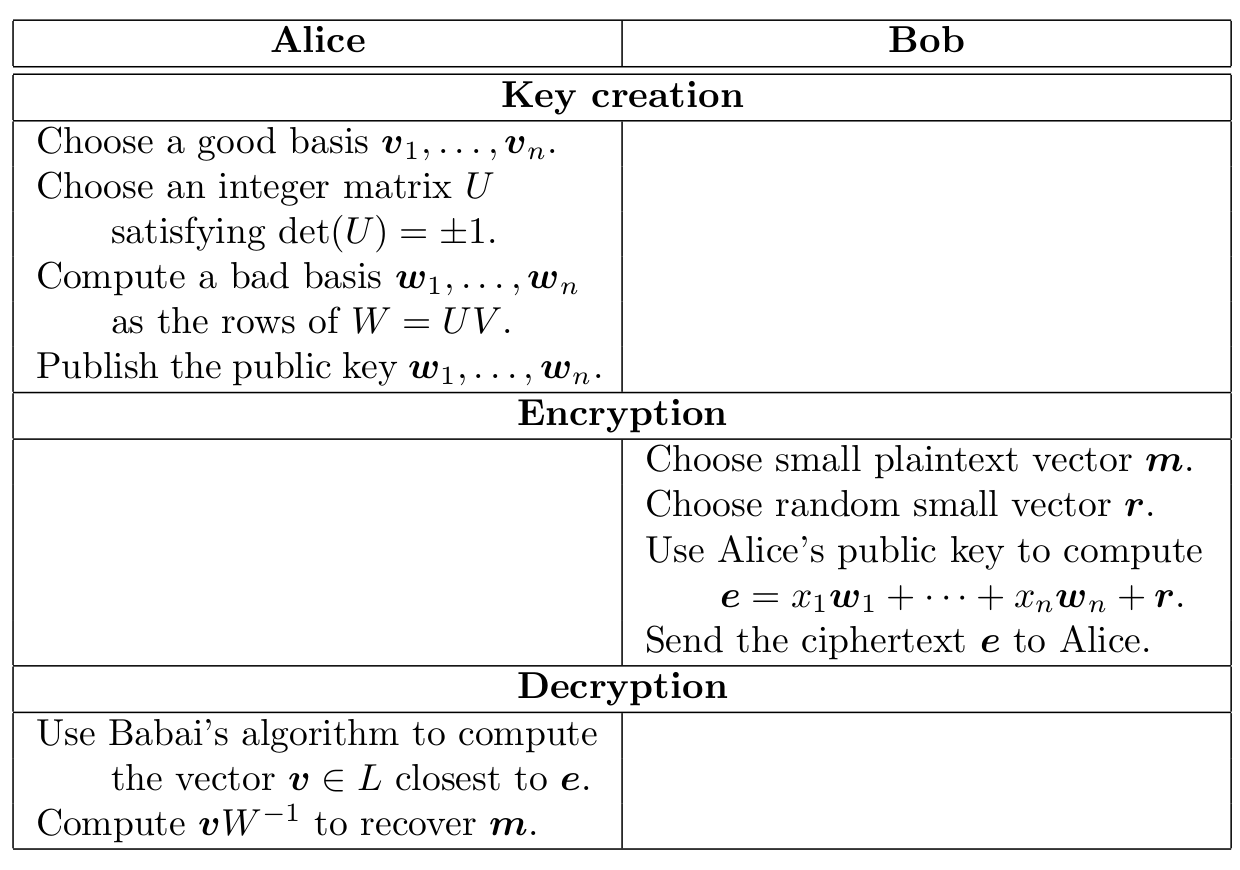
\includegraphics[scale=.2]{GGH.png}

According to Wikipedia, "1999 Nguyen showed at the Crypto conference that the GGH encryption scheme has a flaw in the design of the schemes. Nguyen showed that every ciphertext reveals information about the plaintext and that the problem of decryption could be turned into a special closest vector problem much easier to solve than the general CVP."

\subsection{NTRUEncrypt}

\subsubsection{Convolution Polynomial Rings}
The \textit{ring of convolution polynomials (of rank N)} is the quotient ring
$$R=\frac{\mathbb{Z}[x]}{(x^N-1)}$$ 
This can be interpreted by considering that $\mathbb{Z}[x]$ "introduces x to the integers," but x has no distinguished properties. By taking the quotient $x^N-1$, we're really declaring that $x^N-1=0$, which implies $x$ now has the structure of a root of unity. So really, this ring is just adding an $N$th root of unity, $x$, to the integers.

Another interpretation is that powers of $x$ may be reduced modulo $N$. Multiplication in $R$ reduces to a special case called \textit{convolution}. If we denote the coefficients of polynomials $a(x),b(x)\in \mathbb{R}$ as $(a_0,a_1,\ldots,a_{N-1})$ and $(b_0,b_1,\ldots,b_{N-1})$, then the product is given by
$$a(x)\star b(x)=c(x),\text{ where } c_k=\sum_{i+j\equiv k \mod N}a_ib_{k-i}$$
We frequently work in $R_q$, where the coefficients are modulo $q$. Mapping $R$ into $R_q$ is done in the typical sense. Lifting polynomials from $R_q$ to $R$ is done by selecting the representative whose coefficients are in the interval
$$-\frac{q}{2}<a_i\leq \frac{q}{2}$$
This choice is called the \textit{center-lift}. Note that lifting is not a homomorphism.

\begin{remark}
Let q be prime. Then $a(x)\in R_q$ has a multiplicative inverse if and only if
$$\text{gcd}(a(x),x^N-1)=1\: \text{ in }(\mathbb{Z}/q\mathbb{Z})[x]$$
In this case, the inverse can be calculated using the extended Euclidean algorithm, since there exists $u(x),v(x)\in(\mathbb{Z}/q\mathbb{Z})[x]$ such that
$$a(x)u(x)+(x^N-1)v(x)=1$$
and thus $a(x)^{-1}=u(x)$ in $R_q$.
\end{remark}

\subsubsection{NTRUEncrypt Cryptosystem}
We define the set

$$\mathcal{T}\left(d_{1}, d_{2}\right)=\left\{\begin{array}{ll}
& a(x) \text { has } d_{1} \text { coefficients equal to } 1 \\
a(x) \in R: & a(x) \text { has } d_{2} \text { coefficients equal to }-1 \\
& a(x) \text { has all other coefficients equal to }0
\end{array}\right\}$$
Every \textit{ternary polynomial} (a polynomial whose coefficients are 1, -1, or 0) is in some $\mathcal{T}(d_1,d_2)$.

The fundamental process of NTRU is as follows:

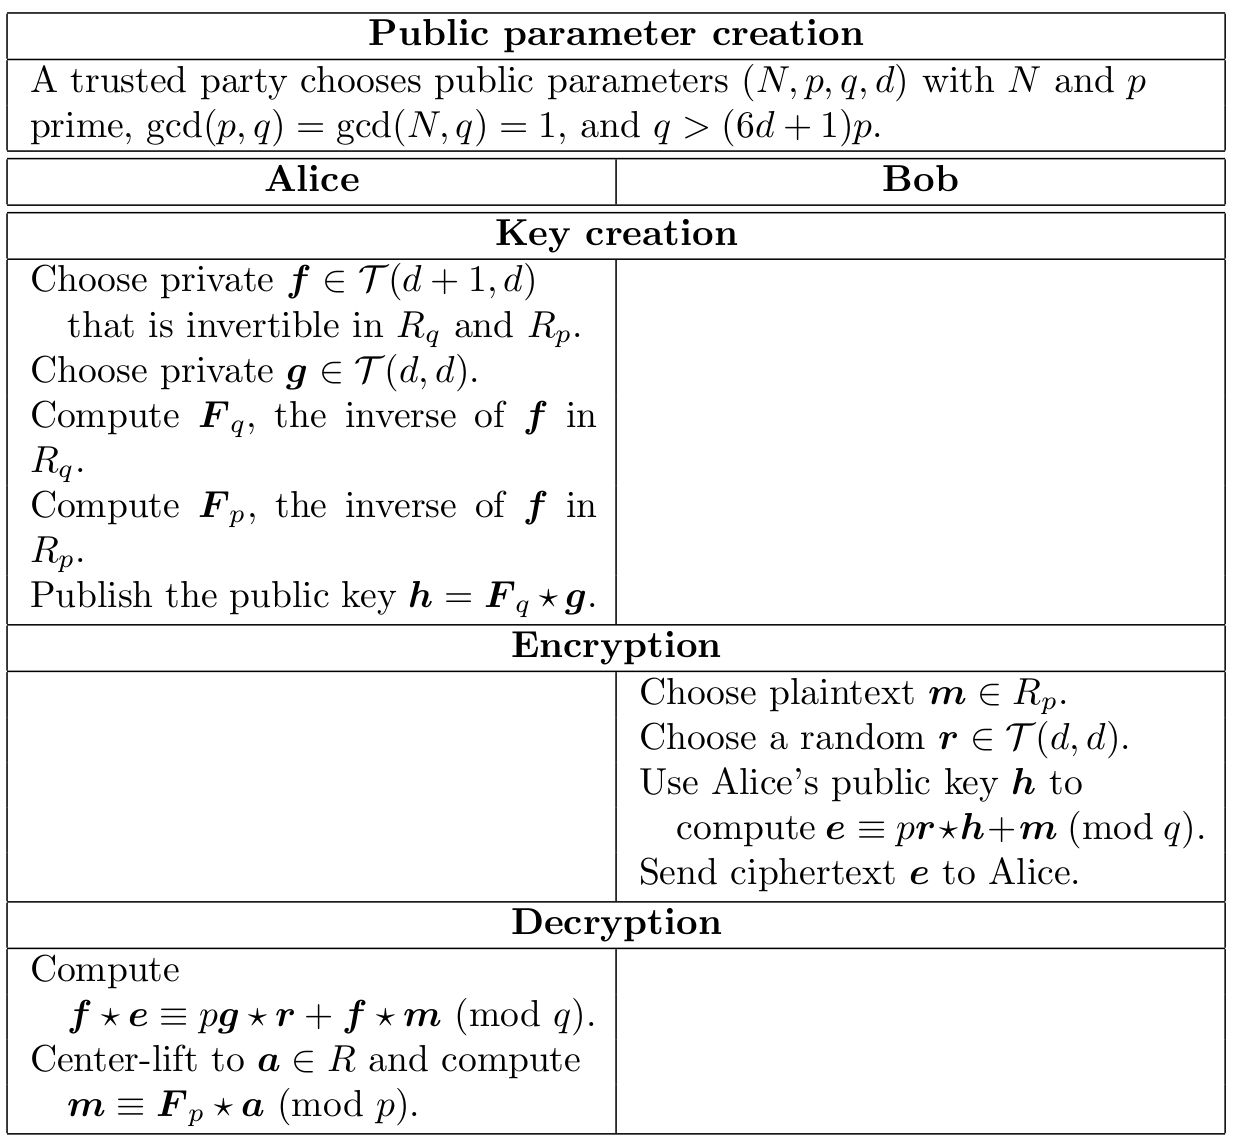
\includegraphics[scale=.2]{NTRU.png}

It's important to consider what is happening in the Decryption step. When we lift $f\star e\equiv pg\star r + f\star m$, the largest coefficient possible is $\left(3d+\frac{1}{2}\right)p$. Because we assumed $q>(6d+1)p$, it follows the coefficients are totally preserved by center-lifting. This is the reason that the noise is then eliminated modulo p.

One cannot simply take the modulo q equation modulo p. The modulo q "breaks" the divisibility of the noise by p. Additionally, one cannot immediately lift the ciphertext, since this will not recover the divisibility of the noise by p. It's essential that you first use $f$ to simplify everything back to polynomials with small coefficients.

So, intuitively, an attacker would be looking for a polynomial f which makes the coefficients of the polynomial small.

Fun observation: the polynomial $f(x)\in\mathcal{d+1,d}$ has small coefficients, but the coefficients of its inverse $F_q(x)$ tend to be randomly and uniformly distributed modulo q. This is an experimental fact. How convenient! This implies that the search for our f can't be narrowed down to a certain region.

The book rephrases the attacking side by noting that, given the assumption $g$ and $f$ are small ternary polynomials, we're looking for some $f$ such that $f(x)\star h(x)$ is also ternary modulo q. 

\subsection{Questions}
\begin{itemize}
\item In what way is GGH flawed?
\item What do homomorphic lifts look like? Do they exist? (Probably not, excepting the trivial case).
\item Can $N$ divide $q$? Why can't it divide $p$?
\item Why do we use $\mathcal{T}(d_1,d_2)$? Is it because these are essentially "good" bases of a lattice? 
\end{itemize}

\end{document}